% Chapter Template

\chapter{Conclusion} % Main chapter title
\label{Chapter7} % Change X to a consecutive number; for referencing this chapter elsewhere, use \ref{ChapterX}
\lhead{Chapter 7. \emph{Conclusion}} 
\section{Project Summary}
In this section summary of the Indriya platform is described
\subsection{System specification}
 The Indriya platform could be seen as a product by itself. The prduct specification is shown in Table~\ref{table:system}.
\begin{table}
\centering
%\footnotesize
\caption{Indriya Specification}
\label{table:system}
\begin{tabularx}{\textwidth}{X X X}
\toprule
  \multirow{2}{*}{Hardware} & Supported Robots & Nao \\
                            & Sensor & Kinect for Windows V2 \\
                            & PC & 64-bit (x64) processor, min 4GB Memory, Physical dual-core 3.1 GHz or more,USB 3.0 controller, DX11 capable graphics adapter\\
                                          \toprule                                       
  \multirow{2}{*}{Software} & Platform & Windows 8.1  \\
                            & For running & Microsoft .NET 4.5.1, Visual C++ Redistributable Kinect SDK, Choreographe, Kinect for Windows SDK \\
                            & For developing & Visual studio community 2013, See readme for list of dependencies \\
                                          \tabularnewline\toprule
\end{tabularx}
\end{table}
The Table~\ref{table:platform_revisited} clarifies the functionalities of Indriya platform.

\begin{table}[H]
\centering
\small
\caption{Indriya platform revisited}
\label{table:platform_revisited}
% \begin{tabular}{|l|l|p{1cm}|p{1cm}|p{1cm}|p{1cm}|p{3cm}|}
\begin{tabular}{|r|p{10cm}|}
\hline
  \textbf{$What is it?$}  & \begin{itemize}
                            \item Design behavior programs
                            \end{itemize}
  \tabularnewline \hline
  \textbf{$What is it not?$}  & -
  \tabularnewline \hline
\end{tabular}
\end{table}
	
The source code of the complete Indriya is available as Open source at \url{https://github.com/praveenv4k/Indriya}. 
\subsection{Project Statistics}

\begin{table}[h!]
  \begin{center}
    \caption{Project Code Statistics}
    \label{table:code_stats}
    \pgfplotstabletypeset[
      columns = {language,comment,code},
      multicolumn names, % allows to have multicolumn names
      col sep=comma, % the seperator in our .csv file
      %display columns/0/.style={
      %    column name=$Files$, % name of first column
      %    column type={S},string type
      %},  % use siunitx for formatting
      %display columns/0/.style={
      %    column name=$Files$,
      %    string type
      %},  % use siunitx for formatting
      display columns/0/.style={
        column name=$Language$,
        string type
      },
      %display columns/1/.style={
      %  column name=$Blank$,
      %  string type
      %},
      display columns/1/.style={
        column name=$Comment$,
        string type
      },
      display columns/2/.style={
        column name=$Code$,
        string type
      },
      every head row/.style={
        before row={\toprule}, % have a rule at top
        after row={
          %\si{\ampere} & \si{\volt}\\ % the units seperated by &
          \midrule} % rule under units
      },
      every last row/.style={after row=\bottomrule}, % rule at bottom
    ]{assets/cloc_code_statistics.csv} % filename/path to file
  \end{center}
\end{table}

\begin{tikzpicture} 
\pie[text=legend]{43.85/C\#, 22.83/C++, 9.52/Python, 6.96/Javascript, 16.8/Others} 
\end{tikzpicture}

\begin{figure}
\centering
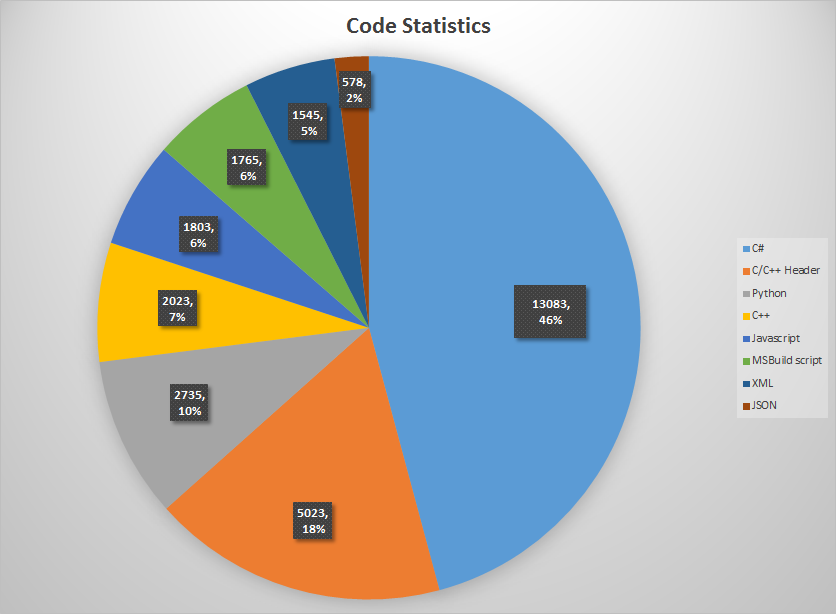
\includegraphics[width=0.8\textwidth]{assets/code_statistics.png}
\caption{Code Statistics}
\label{fig:code_stats}
\end{figure}  

\subsection{Scope for prospective work}
  The Indriya platform has tremendous hope for future developments. Some of the directions that could be thought are

\begin{itemize}
\item Integration of sensors available in smartphone and wearable devices like IMUs, Gyroscopes, GPS etc.,
\item Integration of Natural Language Processing systems with the speech recognition module for more natural interaction
\item Increasing the range of operation of Humanoid robots by fusing data from two or more Kinect sensors 
\item Support for social behavior learning and intelligence modules for dynamic adoption of human like behavior by robots
\end{itemize}

\section{Conclusion} % Main chapter title
	Human Robot Interaction is a complex interdisciplinary problem that needs expertise in various fields like human computer interaction, psychology, biomechanics, humanoid robotics etc., Social robots have become very common in the recent days and they find useful applications in entertainment, education, autism treatment and elderly care. 
	
	For an efficient interaction with human, the robot has to understand his motions and also the environment around him. This is only possible when the robot has necessary perception capabilities which seemlessly make the robot understand the human motions. However the onboard sensors most often cannot deliver all the information necessary for an effective interaction. So there is a need to augment exteroceptive sensors to the system and RGB-D sensors prove to be a convincing solution to this purpose. Irrespective of the underlying perception system used, there is also a need for a scalable robot behavior design framework which could take care of automatic information flow between various components in the system and dynamic creation of behaviors based on object permanence in the environment. Combining the perception system and behavior framework will result in a platform wherein interaction based on human motion will be possible. 
	
	This bibliographic study explained the requirements and challenges in each of the problems of motion understanding, robot localization, behavioral design and evaluation techniques. The state of the art research helped to make appropriate choices to tackle each of the problems under study. More specifically in the research plan described in this study, it is proposed to use Kinect V2 sensor as the perception system and use of Kinect SDK for human motion understanding. The robot localization and tracking problem will be tackled by using a parallelized implementation of particle filter tracking algorithm available in Point cloud library. The Target Drives Means(TDM) framework will be used as the dynamic behavior design infrastructure. An example TDM program is also presented that uses the aforementioned experimental platform. The state of the art HRI evaluation techniques like self assesments and behavioral measures will be used to evaluate the interaction. The experimental platform this thesis aims to achieve will encourage diverse experiments focusing on the evaluation of specific interaction metrics.